\documentclass[12pt,a4paper,titlepage]{report}

\usepackage{times}

\usepackage[utf8]{inputenc}
\usepackage[T1]{fontenc}
\usepackage[romanian]{babel}

\usepackage{setspace}
\onehalfspacing

\usepackage[hidelinks]{hyperref}

\usepackage{graphicx}

\usepackage{minted}
%TODO: remove red box on parser error

\setminted{baselinestretch=1,fontsize=\footnotesize}

\usepackage{caption}

\author{Barbu Paul - Gheorghe}

%TODO: coperta
%TODO: plan tematic?

\begin{document}

\begin{titlepage}
{
\centering
UNIVERSITATEA "LUCIAN BLAGA" DIN SIBIU\\
FACULTATEA DE INGINERIE \\
DEPARTAMENTUL DE CALCULATOARE ŞI INGINERIE ELECTRICĂ\\
}

\vfill

{
\centering
\Large
Secured Bootloader: program pentru controlul secvenței de
inițializare și al actualizării aplicației în microcontrollere
programabile
}

\vfill
{
\raggedright
Conducător ştiinţific: TODO: c.d. cu  grad şi titlul de doctor \\
Îndrumător: TODO: c.d. ce s-a ocupat de student
}
\vfill

{
\raggedright
\hspace*{160pt}Absolvent: \\
\hspace*{160pt}Barbu Paul - Gheorghe\\
\hspace*{160pt}Specializarea:\\
\hspace*{160pt}Calculatoare și Tehnologia Informației
}

\end{titlepage}

\tableofcontents
\newpage

\subsection*{Prezentarea temei}

Lucrarea de față își propune dezvoltarea unui bootloader securizat pentru dispozitive embedded, aceste dispozitive conțin un microcontroller și în general utilizatorul respectivelor dispozitive nu vede și nu interacționează direct cu microcontroller-ul. Exemple de dispozitive embedded sau de aparate care conțin asemenea dispozitive: frigider, mașină de spălat, autoturism, termostat, contor electric, sistem de alarmă, sistem de supraveghere, ceasuri, etc.

Un bootloader este o aplicație care este în general încărcată pe microcontroller de către firma care vinde microcontroller-ul și care nu poate fi înlocuită ușor de către utilizatorii acestuia.
Rolul acestei aplicații este de a fi gazda ("host"-ul) și de a face verificările necesare încărcării unei alte aplicații pe microcontroller. În urma verificărilor se poate afirma că aplicația "guest" sau utilizator este una validă și că poate fi rulată de microcontroller cu încredere.
În urma procesului de bootloading ambele aplicații, atât bootloader-ul cât și aplicația utilizator, vor coexista în
memoria non-volatilă a dispozitivului embedded\footnote{în general pe flash-ul microcontroller-ului, conform unui memory map predefinit de producător}.
 
Motivele pentru care bootloader-ul este securizat și pentru care înlocuirea lui sau a aplicației utilizator
nu ar trebui să poată fi făcută de oricine țin în mică parte de protejarea proprietății intelectuale a celor ce creează aplicații guest pentru respectivul dispozitiv și într-o mai mare măsură țin de asigurarea integrității și a evitării modificării neautorizate a acestei aplicații pentru a asigura utilizatorului experiența pe care producătorul dispozitivelor embedded și-a imaginat-o. Acest lucru este crucial în ziua de astăzi, când criminalitatea în mediul cibernetic este în creștere\cite{interpol}\cite{morgan2016}. Consumatorii trebuie să poată fi protejați proactiv de acțiunile ilegale ale crackerilor, în antiteză cu metoda tradițională, reactivă care constă în schimbarea și îmbunătățirea unui sistem după ce acesta a fost compromis. Cele două metode se complementează reciproc, dar metoda proactivă are avantajul prevenirii unei acțiuni malițioase asupra sistemului informatic.

În afară de îmbunătățirea securității unui sistem embedded precum a fost descris mai sus, rolul bootloader-ului ar trebui să fie și de a mări flexibilitatea unui astfel de sistem. Acest rol este îndeplinit prin faptul că aplicația utilizator de pe microcontroller poate fi schimbată fără modificări hardware asupra sistemului. Schimbarea aplicației utilizator poate surveni din diverse motive, printre care: dezvoltatorul sistemului embedded hotărăște că este timpul să introducă funcționalități noi în aplicație sau că aplicația veche are unele defecte (bug-uri) care trebuie reparate sau chiar că sistemul embedded care înainte îndeplinea un rol trebuie să îndeplinească un rol complet nou, diferit față de cel vechi. Toate aceste scenarii implică folosirea bootloader-ului pre-instalat pe un dispozitiv pentru a încărca o altă aplicație (fie că e una complet nouă sau doar puțin modificată datorită remedierii defectelor din versiunea anterioară).

Bootloader-ul dezvoltat ar trebui să ne permită de asemenea reducerea costurilor. Prin costuri putem să considerăm de exemplu costurile survenite în urma livrării unui sistem embedded. Prin definiție mecanismele interne ale unui astfel de sistem nu sunt accesibile consumatorilor, deci orice modificare, fie ea chiar și software trebuie să fie făcută de producător. Așadar dispozitivul trebuie să fie livrat la producător, acesta aplică modificările și livrează înapoi dispozitivul clientului. Prin intermediul bootloader-ului ne propunem să putem face aceste modificări software la distanță. În esență aceste modificări se vor putea face independent de către fiecare utilizator al sistemului.

Succint cerințele pe care trebuie să le satisfacă bootloader-ul sunt:
\begin{itemize}
\item asigurarea flexibilității dispozitivului embedded prin faptul ca aplicațiile de utilizator se pot schimba la nevoie
\item asigurarea securității și integrității unui sistem embedded în momentul în care aplicația este încărcată\footnote{securitatea sistemului depinde 100\% de aplicație în momentul în care aceasta rulează}
\item minimizarea costurilor de întreținere a dispozitivelor embedded dintr-un mediu industrial prin posibilitatea de a acționa bootloader-ul din exteriorul sistemului embedded
\end{itemize}

Prin rezolvarea acestor puncte, bootloader-ul va fi de ajuns de generic pentru aplicabilitate în diverse domenii și pe diverse platforme hardware. Fiind vorba de mediul embedded, bootloader-ul a fost proiectat și dezvoltat cu constrângerile de mărime în minte, cu atât mai mult cu cât pe un microcontroller se vor stoca două aplicații simultan, bootloader-ul și aplicația utilizator, dar doar una va rula la un moment dat.

\newpage
\chapter{Considerații teoretice}
\section{Introducere și etimologie}
Un bootloader se află pe orice sistem de calcul care trebuie să încarce un sistem de operare sau o aplicație terță.
Acest lucru este valabil fie că utilizatorul interacționează cu sistemul în timpul procesului de "boot" fie că procesul se petrece automat, fără interacțiune umană.

Cuvântul bootloader vine de la procesul de "boot" (sau "boot up"), care la rândul său este o scriere prescurtată a "bootstrap". Bootstrap în engleză semnifică "to pull oneself up by one's bootstraps", procesul prin care noi pornim la drum încălțându-ne. \cite{wikiBootstrap}

\section{Modul de funcționare al unui bootloader}
Orice bootloader trebuie stocat într-o memorie non-volatilă și de preferat disponibilă doar pentru citire, o memorie ROM\footnote{Read-Only Memory}, deoarece acesta trebuie să fie disponibil în momentul în care sistemul pornește indiferent de ce s-a întâmplat anterior pe sistem. Acest lucru garantează funcționarea corectă a sistemului și faptul că sistemul de operare sau aplicația utilizator poate fi schimbată. În caz contrar, când sistemul încetează să funcționeze din cauza unui defect (în general software) putem spune ca este "brick-uit", de la englezescul "brick" (cărămidă)\cite{wikiBrick}.

Un bootloader este, fără excepție, primul program executat de către un procesor, bine-înțeles cu excepția BIOS-ului\footnote{Basic Input/Output System} pe x86, dar putem ignora această particularitate, deoarece pe sistemele embedded, noțiunea de BIOS nu există.
În linii mari codul bootloader-ului este încărcat de pe discul solid\footnote{ROM la dispozitive embedded} în RAM\footnote{Random - Access Memory}, apoi este executat, iar în urma execuției acestui cod (în mod tipic un sector) se poate întâmpla unul din două lucruri:
\begin{enumerate}
\item bootloader-ul și-a încheiat treaba și a predat controlul aplicației utilizator respectiv sistemului de operare
\item bootloader-ul nu încape într-un sector și codul executat anterior este doar auxiliar
\end{enumerate}
Prima variantă este cea trivială. În al doilea caz avem de a face cu un așa zis "two stage bootloader", în primul stagiu făcându-se doar apelul spre acest stagiu secundar. Aici se va face de fapt încărcarea aplicației utilizator. Motivul din spatele încărcării în două faze este faptul că, fără drivere de disc și fără sisteme de fișiere, unitatea maximă pe care procesorul o poate citi de pe hard disc este sectorul, așadar intervin limitări legate de mărimea codului care poate fi executat la un moment dat.

Posibila diferență la sistemele embedded este aceea că microcontroller-ul poate executa cod direct din memoria flash și că bootloader-ul este probabil mai mic ca un sector, deoarece aplicațiile sunt reduse ca dimensiune și ca periferice cu care pot interacționa, display-ul și tastatura nefiind necesare în astfel de sisteme în timpul procesului de boot up.

La calculatoarele personale un bootloader bine cunoscut și pentru care avem nevoie de display și tastatură este GNU GRUB, folosit de majoritatea distribuțiilor GNU/Linux. Acest bootloader este vizibil utilizatorului (pe ecran, prin intermediul unui meniu asemănător cu cel din figura \ref{grub2menu}), iar în cazul sistemelor dual-boot sau multi-boot se poate chiar schimba sistemul de operare ce urmează a fi încărcat, acest lucru se face folosind tastatura.
\begin{figure}[h]
    \centering
    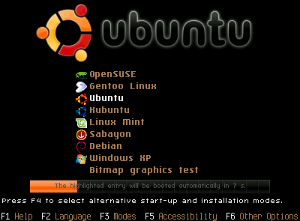
\includegraphics{grub}
    \caption{Meniul GRUB2}
    \label{grub2menu}
\end{figure}

\section{Studiu de caz: secvența de boot la PC}
Deși nu este în domeniul bootloader-ului, datorită omniprezenței acestor tipuri de procesoare merită să ne familiarizăm cu secvența de pași pe care un procesor din familia x86 o execută atunci când este pornit.
Această secvență fiind în strânsă relație cu pornirea bootloader-ului.

La pornire procesorul intră în modul real și execută instrucțiunea de la adresa \texttt{0xFFFFFFF0}\footnote{pe sisteme 32 si 64 bit} \cite{intel80386} \cite{intel64}. În mod normal această locație conține o instrucțiune de salt la locația de start a BIOS-ului care se află într-o memorie ROM.
BIOS-ul este de fapt primul program care se execută pe această arhitectură, nu direct bootloader-ul, în contradicție cu ceea ce am precizat anterior. Rolul BIOS-ului este de a inițializa hardware-ul și de a-l abstractiza, acesta rămânând tot timpul în funcțiune \cite{wikiBootSeq}.

Pasul de inițializare făcut de BIOS, poartă denumirea de POST\footnote{Power-On Self Test}, pas în care BIOS-ul pregătește memoria RAM și bus-urile pentru a putea începe comunicația cu perifericele a căror prezență urmează să o verifice. Aceste verificări sunt necesare, deoarece contrar unui sistem embedded, într-un calculator personal pot apărea și dispărea componente de la o pornire la alta, de exemplu putem adăuga o placă de rețea sau putem scoate placa video dedicată, în oricare dintre aceste cazuri BIOS-ul trebuie să știe de prezența unui periferic nou sau de lipsa unuia vechi pentru a putea prezenta toate aceste informații nivelelor superioare, care vor pune în funcțiune perifericele respective.
\begin{figure}[h]
    \centering
    \includegraphics{structuraPC}
    \caption{Structura "cochilie" a PC-ului}
    \label{shellArchitecture}
\end{figure}
Se poate observa în figura \ref{shellArchitecture} că BIOS-ul abstractizează hardware-ul, acest lucru este făcut mai departe și de sistemul de operare prin intermediul driverelor și prin intermediul apelurilor de sistem\footnote{"syscalls" sau "system calls" în engleză}. Datorită poziționării lor în centrul cochiliei, din aceeași figură reiese că aplicațiile beneficiază de cel mai mare nivel de abstractizare, ele nu trebuie să știe detalii intime despre așezarea datelor pe hard disk, în schimb au la dispoziție conceptul de fișier, indiferent de câte sectoare ocupă un asemenea fișier sau cum se comandă citirea lui la nivelele inferioare ale arhitecturii.

După inițializarea perifericelor, BIOS-ul trece printr-o listă pre-configurată de dispozitive de stocare non-volatile
până când găsește unul boot-abil. Un asemenea dispozitiv este caracterizat de faptul că ultimii doi octeți ai primului sector sunt egali cu \texttt{0x55AA}, aceasta reprezentând "semnătura" unui disc boot-abil.
Cel mai probabil această secvență \texttt{0x55AA} a fost aleasă deoarece în binar ea arată așa: \texttt{0101 0101 1010 1010}, observăm că biții sunt destul de variați, schimbarea în cascadă a lor neproducând din nou aceeași valoare și putând evita astfel încărcarea unui sector invalid sau corupt.

Odată ce discul boot-abil a fost găsit, primul lui sector este încărcat în memorie și executat, aici se află în sfârșit bootloader-ul. Codul este încărcat la adresa \texttt{0x0000:0x7C00} \cite{biosMBRaddr}.

În urma execuției bootloader-ul poate alege în mod automat de unde încarcă sistemul de operare sau, în cazul multi-boot, pasează această responsabilitate utilizatorului, punându-l să aleagă sistemul de operare dorit dintr-o listă.

În acest prim sector se află MBR-ul\footnote{Master Boot Record}. În cele mai multe cazuri cu o dimensiune de 512 octeți, MBR-ul conține de fapt codul bootloader-ului și detalii despre partiționarea discului\cite{norton99}. Codul bootloader-ului poate fi acela al lui GRUB sau bootloader-ul instalat de sistemele de operare Windows.

Structura MBR-ului este prezentată în tabelul \ref{mbrStruct}.

\begin{table}[h]
    \begin{tabular}{ | c | c | c | }
        \hline
        \textbf{Adresă} & \textbf{Descriere} & \textbf{Mărime (octeți)} \\ \hline
        \texttt{0x000} & Codul bootloader-ului & 446 \\ \hline
        \texttt{0x1BE} & Prima tabelă de partiție & 16 \\ \hline
        \texttt{0x1CE} & A doua tabelă de partiție & 16 \\ \hline        
        \texttt{0x1DE} & A treia tabelă de partiție & 16 \\ \hline
        \texttt{0x1EE} & A patra tabelă de partiție & 16 \\ \hline
        \texttt{0x1FE} & Primul octet al semnăturii discului (\texttt{0x55}) & 1 \\ \hline
        \texttt{0x1FF} & Al doilea octet al semnăturii discului (\texttt{0xAA}) & 1 \\ \hline
    \end{tabular}
    \centering
    \caption{Structura MBR-ului}
    \label{mbrStruct}
\end{table}

Din tabelul \ref{mbrStruct} se poate observa de asemenea că bootloader-ul este în realitate constrâns la mai puțin de 512 octeți, deoarece MBR-ul conține atât semnătura unui disc boot-abil, folosită de BIOS, cât și informații despre partițiile primare existente pe mediul de stocare. Pe scurt, tabelele de partiții au structura din tabelul \ref{partitionTableStruct} \cite{wikiPTE} și ele indică unde începe și unde se termină o partiție pe disc, cât și tipul acesteia și faptul că ea conține sau nu un sistem de operare, informație folosită apoi de bootloader pentru a popula lista de sisteme de operare disponibile pe calculator. Așadar dacă bootloader-ul, în urma inspectării tabelelor de partiții, găsește doar una activă, o va alege automat, în caz contrar îi va prezenta utilizatorului o listă cu sistemele de operare (respectiv partițiile pe care se află acestea) spre a face alegerea.

\begin{table}[h]
    \begin{tabular}{ | c | p{8cm} | c | }
        \hline
        \textbf{Adresă} & \textbf{Descriere} & \textbf{Mărime (octeți)} \\ \hline
        \texttt{0x0} & Partiție activă sau nu (conține sau nu un sistem de operare) & 1 \\ \hline
        \texttt{0x1} & Adresa Cilindru-Cap-Sector de început a partiției & 3 \\ \hline
        \texttt{0x4} & Tipul partiției & 1 \\ \hline
        \texttt{0x5} & Adresa Cilindru-Cap-Sector de final a partiției & 3 \\ \hline
        \texttt{0x8} & Adresa logică a blocului (LBA) de început a partiției & 4 \\ \hline
        \texttt{0xC} & Numărul de sectoare al partiției & 4 \\ \hline
    \end{tabular}
    \centering
    \caption{Structura sumară a unei tabele de partiție}
    \label{partitionTableStruct}
\end{table}

Observăm că toate aceste detalii teoretice cu privire la modul de funcționare al unui bootloader și al secvenței de inițializare la sistemele Intel x86 provin din limitarea intrinsecă a bootloader-ului la numai câteva sute de bytes de cod executabil. Pentru a ocoli această limitare s-a dezvoltat bootloader-ul în două stagii. Totuși în sistemele mai noi s-a dezvoltat standardul UEFI\footnote{Unified Extensible Firmware Interface: \url{http://www.uefi.org/}}. Acesta specifică 
un înlocuitor pentru BIOS și poate fi folosit pe o gamă mai largă de arhitecturi, inclusiv ARM, ARM64 și Itanium\cite{uefiSpec}. Este la latitudinea companiilor care comercializează sisteme de calcul să implementeze acest standard, care nu mai are limitările specifice BIOS-ului, acesta putând lucra direct cu fișiere și asigură extensibilitatea procesului de boot,  nu prin încărcarea succesivă a codului în două etape, ci prin aplicații care apelează și respectă interfața standard UEFI, similar unui sistem de plugin-uri.
Spre exemplu UEFI permite pornirea unui terminal de depanare, în cazul în care sistemul nu bootează se pot face investigații direct de la nivelul firmware-ului. De asemenea UEFI permite așa numitul "secure boot" \cite{uefiSpec} care permite încărcarea doar sistemelor de operare cu o semnătură digitală validă, acesta fiind un mecanism de protecție împotriva rulării unui sistem de operare modificat în scopuri malițioase, dar poate fi folosit și ca mecanism de împiedicare a instalării altor sisteme de operare care nu sunt vândute de un anumit producător deoarece acele sisteme de operare nu vor fi validate de mecanismul securizat de boot al UEFI \cite{zdnetSecureBoot}.

\subsection{Variante de bootloader}

În afară de bootloader-ul instalat de sistemele de operare Windows, numit Windows Boot Manager, și de GNU Grub, ambele prezentate anterior, mai există și alte variante de bootloader-e care pot fi instalate pe un sistem de calcul.

Toate aceste bootloader-e diferă în mărime și in funcționalitate, dar în final, toate au același scop: de a găsi și de a porni un sistem de operare.

Sistemul de operare poate fi localizat pe rețea, de exemplu Grub și Syslinux au capabilitatea de a încărca sistemul de operare dintr-o locație centralizată, lucru util în cazul în care un administrator de sistem dorește controlul asupra mai multor sisteme, fără să le administreze manual pe fiecare în parte.

De asemenea anumite bootloader-e pot încărca aplicații sau sisteme de operare comprimate, stocate așa deoarece este posibil ca spațiul să fie limitat, cum este cazul sistemelor embedded. Pentru aceste sisteme a fost dezvoltat bootloader-ul "Das U-Boot" \footnote{http://www.denx.de/wiki/U-Boot/} care poate fi folosit pe o multitudine de arhitecturi și care se axează pe minimizarea mărimii codului și a timpilor de rulare prin simplitatea codului\footnote{http://www.denx.de/wiki/U-Boot/DesignPrinciples}. Urmărirea acestor principii de dezvoltare au făcut ca acest bootloader să fie prezent într-o gama largă  de produse, de la dispozitive industriale, până la echipamente de rețea, cum ar fi cele de la Ubiquiti Networks cât și la laptop-urile dezvoltate de Google, Chromebooks \cite{wikiUboot}.

\section{Studiu de caz: secvența de inițializare la un sistem embedded}

În ceea ce privește sistemele embedded, acestea fiind mai puțin performante față de un calculator personal, putem spune că și secvența de inițializare a lor și respectiv bootloader-ul sunt mai puțin complexe.
Acest lucru este datorat și tipurilor de periferice și dispozitive de stocare cu care sistemul este dotat. În cazul dispozitivelor embedded perifericele ca tastatura sau mouse-ul și monitorul, nu există, iar mediile de stocare sunt in general memorii flash, nu hard disk-uri, făcând accesul la date mult mai simplu și nefiind nevoie de nivelele de abstractizare pe care le oferă BIOS-ul și sistemul de operare.

În general când lucrăm cu un microcontroller, nu există conceptul de bootloader, ci doar conceptul de inițializare al hardware-ului, lucru care este deja implementat de către bibliotecile oferite de producător.
Așadar, când un microcontroller este resetat acesta execută câțiva pași bine definiți pentru a executa codul încărcat (flash-uit) de către dezvoltator, procesul este similar cu cel prezentat anterior pentru arhitecturile x86, dar în mare parte este mai simplu. Simplitatea se trage din faptul ca acest cod de inițializare nu trebuie să verifice în mod dinamic existența unor noi periferice sau lipsa unora vechi deoarece sistemul embedded nu este deschis extensibilității pentru utilizator, acesta este mult mai rigid.

Pentru acest studiu de caz vom considera core-ul M7 de la ARM\footnote{https://www.arm.com/products/processors/cortex-m/cortex-m7-processor.php} împreună cu secvența de inițializare aferentă lui.
Ca pentru orice procesor și pentru acest model există o tabela a vectorilor de întrerupere\footnote{IVT - Interrupt Vector Table}, care nu este altceva decât o zonă de memorie care conține la anumite adrese pointeri spre rutinele de tratare a întreruperilor. În cazul core-ului M7 primele două locații din această tabelă sunt valorile inițiale ale registrului Stack Pointer\footnote{abreviat SP} și ale registrului Program Counter\footnote{abreviat PC sau IP (Instruction Pointer)} \cite{kv5x}.
Combinația celor două registre ne permite să putem începe execuția codului, deoarece Program Counter-ul ne indică adresa următoarei instrucțiuni care trebuie executată de către procesor. Stack Pointer-ul ne indică locația în memorie unde se află vârful stivei, zona de memorie folosită pentru a stoca parametrii unei funcții și date despre locația unde trebuie să revenim din funcția apelată.

În listing-ul \ref{ivt-m7} putem vedea, în cod asamblare, modul în care rutinele de tratare a întreruperilor sunt declarate.
\begin{listing}[h]
\begin{minted}{asm}
__isr_vector:
  .long __StackTop
  .long Reset_Handler
  .long NMI_Handler
  .long HardFault_Handler
  .long MemManage_Handler
  .long BusFault_Handler
  .long UsageFault_Handler
\end{minted}

\caption{Începutul tabelei vectorilor de întrerupere}
\label{ivt-m7}
\end{listing}

Prima intrare din acest vector este valoarea inițială a stack pointer-ului, numit aici \texttt{\_\_StackTop}, acesta nu este un pointer spre o rutină de tratare a unei intreruperi, ci are doar rolul de a indica unde începe zona de memorie rezervată stivei. În schimb cea de a doua intrare în interrupt vector table este într-adevăr un pointer spre o astfel de procedură.
Aceasta este apelată de fiecare dată când procesorul primește semnalul de reset. Din acest motiv putem spune ca PC-ul inițial se află pe poziția a doua în tabelă, deoarece el corespunde acestei rutine.

Continuând pe firul execuției în urma resetării microcontroller-ului, rutina \texttt{Reset\_Handler} nu face altceva decât să 
apeleze funcția \texttt{SystemInit} care este responsabilă cu inițializarea cache-urilor și a unității de procesare a numerelor cu virgulă flotantă. În urma acestui apel controlul este redat rutinei \texttt{Reset\_Handler} care mai departe se va ocupa cu copierea secțiunii de constante a codului în memoria RAM și de inițializarea zonei de memorie rezervată pentru heap (folosită când programul alocă dinamic memoria). De asemenea \texttt{Reset\_Handler}-ul continuă cu apelul funcției \texttt{\_\_libc\_init\_array} (care inițializează structurile necesare limbajului C) și în final va apela punctul unic de intrare într-un program, funcția scrisă de dezvoltator: \texttt{main}.
Codul pentru pașii de inițializare se află în fișierul \texttt{startup\_MKV58F24.S} din directorul \texttt{startup} al unei aplicații embedded\footnote{Locația depinde de producătorul microcontroller-ului și de mediul de programare folosit}.

După ce se apelează \texttt{main}-ul, practic controlul îi este predat aplicației scrisă de dezvoltator și secvența de inițializare a luat sfârșit. În afară de memorie și de componentele auxiliare acesteia, cache-urile, alte componente ale microcontroller-ului nu au fost pornite, acest lucru se datorează faptului că responsabilitatea aceasta este predată aplicației . Lucru necesar pentru a consuma cât mai puțină energie posibil, dacă aplicația nu va folosi, spre exemplu, comunicația pe portul serial, nu va inițializa acest port, ceea ce va duce la evitarea consumului de energie fără scop.

\inputminted{asm}{reset_handler.s}
\captionof{listing}{Definiția rutinei Reset\_Handler\label{resetHandler}}

\begin{figure}[h]
    \centering
    \includegraphics[width=0.75\textwidth]{structuraEmbedded}
    \caption{Structura "cochilie" a unui sistem embedded}
    \label{shellEmbedded}
\end{figure}

Secvența descrisă anterior se poate vedea sub formă de schemă logică în figura \ref{shellEmbedded} și sub formă de cod asamblare în listingul \ref{resetHandler}.
Am păstrat în această figură și analogia structurii cochilie pentru a ilustra diferența majoră între un sistem embedded care funcționează pe o arhitectură ARM\footnote{în cazul de față Cortex M7} și arhitectura x86 folosită în calculatoarele personale și server-e. Diferența constă în faptul că în cazul programării dispozitivelor embedded sistemul nu include nivele de abstractizare pe care programatorul nu le cere și de care nu are nevoie în mod explicit. În mod implicit sistemele embedded nu oferă altceva decât biblioteci care ne dau acces la hardware, la registrele microprocesorului. Prin aceste registre se pot controla porturile de comunicație\footnote{UART, SPI, I2C}, se poate scrie sau șterge memoria flash, putem controla convertoarele analog-digitale și pe cele digital-analogice, etc. Bine-înțeles că există producători care oferă un nivel mai ridicat de abstractizare prin biblioteci, un asemenea producător este NXP\footnote{\url{http://nxp.com/}}. Aceste biblioteci ascund lucrul cu registrele microcontroller-ului în favoarea lucrului cu funcții și structuri\cite{ksdk}, ele reprezintă chiar echivalentul BIOS-ului și al colecției de driver-e în sistemele x86, deoarece scopul lor este similar: de a abstractiza hardware-ul pe care aplicația rulează.

Un programator embedded are la dispoziția sa și sisteme de operare, în principal de tipul "real time"\footnote{de timp real}.
Aceste sisteme de operare sunt caracterizate de predictibilitatea lor și de garanțiile puternice pe care le fac legat de timpul în care termină de executat un task\cite{silberschatz}.

Totuși modul în care acestea sunt folosite diferă substanțial față de modul în care sistemele de operare non-real-time sunt folosite. Acest lucru este datorat faptului că un sistem de operare real-time folosit pe o platformă embedded va fi o parte a aplicației scrisă de dezvoltator, nu există deja un mediu pre-definit în care aplicația este creată, ca la sistemele de operare de uz general. Asta înseamnă că sistemul de operare real-time va fi inclus în aplicație la nivelul codului sursă sau link-at static la aceasta, astfel că funcționalitățile lui sunt accesate asemenea funcționalităților unei biblioteci, prin apeluri de funcții și structuri de date, din nou revenind la analogia anterioară, unde bibliotecile țin loc de BIOS, drivere, și acum, chiar și de sistem de operare real-time \cite{freertos}. 

Acest mod de lucru nu este totuși unic industriei embedded, el poate fi observat într-o oarecare măsură și în cadrul așa numitului unikernel. Un unikernel reprezintă o aplicație de uz general \cite{barbu} și un nucleu de sistem de operare, combinate într-o singură unitate funcțională care poate servi drept firmware-ul unui dispozitiv. Față de cazul embedded, unde sistemul de operare era inclus în aplicație (fie la nivel de cod sursă, fie link-at static), aici lucrurile stau invers, aplicația va fi inclusă direct în sistemul de operare de uz general prin linkare statică. Acest lucru duce la efectul secundar de a putea integra o singură aplicație în unikernel, de unde provine și numele, un nucleu de sistem de operare dedicat unei singure aplicații \cite{kantee}.

%TODO: reitereaza ideea asta la capitolul cu practica
După cum am văzut în listingul \ref{resetHandler}, funcția main este chemată direct, fără să se facă o selecție dintr-o colecție de funcții (corespondente unor aplicații) disponibile, similar cu selecția sistemului de operare de către bootloader.
Putem modifica acest lucru prin introducerea unui strat de abstractizare suplimentar. Adică să scriem o aplicație care să fie apelată implicit de către microcontroller, iar apoi această aplicație să joace rolul de bootloader. Bootloader care va fi responsabil cu alegerea unei aplicații pe care să o ruleze și eventual cu validarea acesteia similar cu sistemul UEFI.

În urma alegerii și validării aplicației, bootloader-ul va trebui să îi predea controlul acesteia, similar unui bootloader pentru arhitecturile x86 care predă controlul sistemului de operare. Totuși fiind vorba de dispozitive embedded rareori este necesar ca bootloader-ul să aleagă între două aplicații guest pe care să le ruleze, așa cum se întâmplă la calculatoarele personale cu bootloader-ul și sistemele de operare. Acest lucru este cauzat de hardware-ul redus ca putere și spațiu de stocare, dar și de o caracteristică intrinsecă a sistemelor embedded: orientarea spre un singur domeniu și rezolvarea unui singur fel de problemă la un moment dat. Așadar este mai probabil ca în bootloader-ele embedded să vedem modalități de a încărca o aplicație complet nouă pe microcontroller (care o înlocuiește pe cea veche) în locul funcționalității de a alege o aplicație dintr-o colecție pre-existentă.

În funcție de tipul microcontroller-ului aplicația se poate încărca folosind un tip de comunicație serială clasică, precum UART, I2C și SPI sau prin metode întâlnite mai des pe sistemele de uz general cum ar fi USB-ul și Ethernet-ul.

\subsection{Variante de bootloader}

Similar arhitecturilor generale, există de asemenea diverse bootloader-e create pentru dispozitive embedded. "Das U-Boot", precizat și în secțiunea anterioară este unul dintre ele, printre principiile acestuia de design aflându-se și portabilitatea.

Printre alte alternative se numără și "KBoot", bootloader-ul celor de la Kinetis. Spre deosebire de "Das U-Boot", acesta este creat special pentru dispozitivele dezvoltate de NXP \cite{kboot}. Procesul de inițializare este similar cu cel descris anterior. Microcontroller-ul pornește și începe să execute codul bootloader-ului, care la rândul său așteaptă să primească o aplicație pe care să o încarce pe toată gama de porturi disponibile pe dispozitiv. În urma încărcării aplicația este pornită. Ceea ce este special la acest bootloader este faptul că el poate fi folosit și drept sistem de control al dispozitivului, permițând rularea unor comenzi administrative cum ar fi citirea anumitor zone de memorie, ștergerea lor și scrierea de date. Bootloader-ul pune la dispoziție și o aplicație similară unui terminal prin care pot fi executate aceste comenzi.

Un alt bootloader embedded este \guillemotleft$\mu$Tasker "Bare-Minimum" Boot Loader\guillemotright, acesta după cum îi spune și numele conține doar minimul necesar pentru a încărca o altă aplicație \cite{uTaskerMinim}. El se bazează pe "$\mu$Tasker Serial Loader" pentru a face încărcarea prin Ethernet, UART sau chiar și de pe carduri de memorie \cite{uTaskerSerial}. Deoarece  încărcarea se face în doi pași, primul făcând minimul necesar și într-un spațiu cât mai mic, iar cel de-al doilea pas făcând încărcarea propriu zisă putem spune că acest bootloader se aseamănă cel mai mult cu bootloader-ele pentru arhitecturi x86, precum GRUB.

\section{Protecția și securitatea}
Unul dintre scopurile pe care bootloader-ul dezvoltat în cadrul acestei lucrări și le propune să le atingă este acela de a asigura integritatea și de a evita modificarea neautorizată a aplicației pe care bootloader-ul o va încărca.

Deducem deci două categorii de modificări care pot surveni asupra aplicației:
\begin{enumerate}
\item modificarea ne-intenționată datorată problemelor de transmisie spre microcontroller;
\item modificarea intenționată, posibil pentru a rula cod malițios.
\end{enumerate}

Vom studia în cele ce urmează posibile soluții pentru aceste două probleme.

\subsection{Coduri polinomiale}
Pentru a preveni prima categorie de modificări, cele datorate mediului de comunicație, soluțiile trebuie să acționeze la nivelul pachetelor care se transferă între microcontroller și calculator (dacă presupunem de exemplu o transmisiune serială, RS232). În timpul transferului de date, datorită interferențelor, anumiți biți pot ajunge schimbați la destinație. Pentru a detecta astfel de erori avem la dispoziție mai multe tehnici.

Cea mai simplă tehnică ar fi introducerea unui bit de paritate de către expeditor, bit pe care destinatarul trebuie să îl verifice pentru a avea siguranța că datele au fost transmise corect. Această tehnică poate detecta schimbarea unui singur bit. Este deci o metodă simplă, nu adaugă meta-date, în afară de bit-ul de paritate, datelor utile. Un exemplu ar fi dacă dorim să transmitem șirul de biți \texttt{0101 1010} cu paritate pară, atunci acesta ar deveni: \texttt{0101 1010 0}, iar cu paritate impară ar deveni: \texttt{0101 1010 1}. Observăm că în primul caz, cel al parității pare, numărul total de biți setați (cu valoarea 1) este par și am adăugat la final un bit de 0, iar în cazul parității impare, numărul transmis de biți cu valoarea 1 este impar deoarece am adăugat la final un bit de 1. Totuși acestă metodă nu este de ajuns pentru a detecta dacă mai mulți biți au fost afectați de erori, după cum se poate vedea în cazul următor: dacă dorim să transmitem secvența de biți \texttt{0101 1010} cu paritate pară vom transmite secvența \texttt{0101 1010 0}. În timpul transmisiei, datorită interferențelor doi biți se modifică din 1 în 0: \texttt{0000 1010 0}, făcând astfel datele care ajung la destinatar să fie diferite față de cele expediate, dar cu un bit de paritate încă valid și drept consecință făcând imposibilă detectarea erorilor.

În urma acestor limitări W. Wesley Peterson a descoperit un algoritm mai complex de detecție a erorilor, numit cyclic redundancy check\footnote{CRC}, "coduri ciclice" sau "coduri polinomiale" \cite{wikiCrc}. Rezultatul acestui algoritm este, similar cu bit-ul de paritate, adăugat datelor utile (de unde vine și denumirea de "redundant", deoarece nu adaugă date noi, ci reprezintă o transformare a celor existente deja). Codurile ciclice sunt mai versatile deoarece acestea pot detecta erori în secvențe mai lungi de un bit. Acest algoritm de detecție al erorilor este folosit și la nivelul "Data Link"\footnote{legătură de date} al modelului ISO-OSI datorită capacității lui bune de a detecta erori.

Rezultatul unui CRC este reprezentat pe un număr fix de biți, de exemplu unele dintre cele mai folosite astfel de coduri polinomiale sunt CRC-8, CRC-16 și CRC-32, cu reprezentări pe 8, 16 și respectiv 32 de biți. Lungimea acestora este aleasă în funcție de cât de bună dorim să fie detecția și de cât de multe meta-date dorim să adăugăm mesajului util. De regulă codul polinomial poate detecta erori de o lungime maximă cu lungimea proprie de reprezentare, de exemplu CRC-32 poate detecta maxim un șir de 32 de biți alăturați care au fost modificați în timpul transferului.

CRC-urile se mai numesc coduri polinomiale deoarece polinoamele sunt fundamentul matematic pe care se bazează. Algoritmul care calculează CRC-ul tratează un șir de biți ca fiind coeficienții unui polinom de ordin n+1.
Așadar șirul de biți \texttt{0000 00111} corespunde polinomului $x^8 + x^2 + x + 1$, prin convenție cel mai semnificativ bit este tot timpul 1 fără să fie reprezentat (aici coeficientul lui $x^8$), de aceea de exemplu algoritmul CRC-8, cu rezultatul reprezentat pe 8 biți are de fapt 9 membrii în polinom. Operațiile aritmetice cu polinoame se fac în "modulo 2", ceea ce înseamnă că nu există carry pentru adunare și împrumuturi pentru scădere. Acest lucru face ca adunarea și scăderea să fie echivalente cu operația de sau-exclusiv \cite{tanenbaumCN}. Pentru a calcula CRC-ul unui șir de biți, atât destinatarul cât și expeditorul trebuie să stabilească un polinom comun pe care să îl folosească la generarea CRC-ului, acest polinom se numește sugestiv: polinom generator. Polinomul generator este folosit ca împărțitor, iar biții datelor utile sunt folosiți pentru a construi polinomul deîmpărțit. În urma operației de împărțire între cei doi termeni, doar restul se va folosi, el este CRC-ul și este reprezentat pe n biți, unde n+1 este ordinul polinomului generator. Este important să subliniem că împărțirea polinoamelor are loc în aritmetică modulo 2, acest lucru făcând facilă implementarea algoritmului de calcul al unui CRC în hardware, acesta necesitând doar registre de shiftare și porți XOR \cite{hackersDelight}.

Din punct de vedere software o funcție în limbajul C care calculează un CRC pe 16 biți este prezentată în listing-ul \ref{crcInC}. Din cod se poate vedea cum pentru fiecare bit, al fiecărui octet din datele de intrare, celui mai semnificant bit al CRC-ului și bit-ului de date le sunt aplicate operația de sau-exclusiv și apoi CRC-ul este shiftat la stânga cu o poziție \cite{rossCrc}.

\begin{listing}[h]
\begin{minted}{c}
uint16_t Crc16(const uint8_t *pu8Data, const uint32_t u32DataLen,
               const uint16_t u16Poly, uint16_t u16Crc)
{
    for(uint32_t byte=0; byte<u32DataLen; ++byte)
    {
        u16Crc ^= (*pu8Data++) << 8;
        for(uint8_t bit=0; bit<8; ++bit)
        {
            u16Crc = (u16Crc << 1) ^ ((u16Crc & 0x8000) ?
                                      u16Poly : 0);
        }
    }

    return u16Crc;
}
\end{minted}

\caption{Implementarea unei rutine de calcul a CRC-16}
\label{crcInC}
\end{listing}

Folosind algoritmul exemplificat în listing-ul \ref{crcInC} atât expeditorul cât și destinatarul vor calcula codul ciclic. Dacă destinatarul observă că valoarea CRC-ului diferă înseamnă că au apărut erori la trimiterea datelor și cere o re-transmisiune până când erorile nu mai apar. Datorită faptului că discutăm despre un sistem embedded codurile de corecție a erorilor nu au fost considerate spre implementare, ci doar cele de detecție a erorilor, prezentate anterior.

\subsection{Encripția și autentificarea datelor}

Unul dintre scopurile bootloader-ului este reducerea costurilor prin acționarea sa "de la distanță". Pentru a face acest lucru dezvoltatorul de aplicații trebuie să îi trimită clientului o aplicație care să fie folosită de bootloader. Bine-înțeles acest lucru se poate face pe internet (de exemplu prin email sau upload pe web), dar expunerea aplicației pe web presupune riscul de a expune aplicația la modificări malițioase. O persoană cu rele intenții poate pune la cale un atac de tip man-in-the-middle\footnote{tradus literalmente: om în mijloc} în care clientul este practic păcălit că descarca aplicația dezvoltatorului, dar de fapt descarcă un virus, care va fi apoi încărcat pe dispozitivul său. Datorită naturii sale embedded dispozitivul ar putea părea că își face treaba pe care a fost proiectat să o facă, dar, în plus, poate să adune și date despre utilizator sau chiar să permită controlul neautorizat asupra dispozitivului. Gradul de gravitate al acestei breșe de securitate diferă în funcție de dispozitiv și de întrebuințarea lui, dar ne dorim totuși să prevenim aceste modificări nedorite ale aplicației.

Trebuie să observăm că de data aceasta modificările aduse aplicației nu mai sunt ne-intenționate, ci intenționate, așadar nu mai putem sa folosim CRC-urile, având nevoie de un sistem dedicat pentru această gamă de probleme. Codurile polinomiale nu sunt o opțiune deoarece, în general, acestea se atașează la finalul datelor utile și pot fi recalculate cu ușurință, un atacator putând să schimbe o porțiune de cod și apoi să recalculeze CRC-ul și să îl înlocuiască pe cel original.

Soluția pe care o căutăm este una de natură criptografică. Pentru a evita orice fel de contact cu mediul exterior aplicația trebuie să fie criptată în momentul în care dezvoltatorul o publică și trebuie să fie decriptată doar pe dispozitivul embedded, de către bootloader. În acest mod dezvoltatorul și clientul pot fi siguri că aplicația nu poate fi modificată deoarece conținutul ei decriptat nu este expus niciodată. Algoritmul de criptare ales este Advanced Encryption Standard - Galois Counter Mode\footnote{AES-GCM} \cite{wikiAes} cu o cheie de 128 de biți deoarece acest algoritm se găsește implementat în biblioteci special create pentru mediul embedded\footnote{\url{https://tls.mbed.org/}} și, dacă este implementat corect, până acum nu s-a descoperit nicio vulnerabilitate practică asupra lui, metodele curente având o complexitate de timp de aproximativ $2^{120}$ \cite{bogdanov}.

%TODO:  https://en.wikipedia.org/wiki/Advanced_Encryption_Standard

TODO: AES (figuri wiki) și pseudo-cod
TODO: why I need GCM and what it is, daca am cheia pot reface aplicatia, dar cu gcm ar trebui sa am si iv-ul.
TODO: GCM vs CRC


TODO: Despre chei si faptul ca acestea trebuie scrise pe dispozitiv, tocmai ca sa nu vada lumina zilei.
TODO: Spune cum faptul ca cheile se afla pe dispozitiv nu este o problema pt. ca flash-ul trebuie sters cand este securizat, detalii in sectiunea viitoare.

\section{Procesul de flashing al unui microcontroller}
TODO: securitatea flash-ului, reference Using the Kinetis Security and
Flash Protection Features
TODO: scrie-ma, despre JTAG, stergerea flash-ului, tehnologii de flash, el de fapt este pe 1 si cand scriem se duce pe 0

\newpage
\chapter{Rezolvarea temei de proiect}
\section{Introducere}

TODO: despre cum se scrie codul in lumea embedded, fara bootloader prima data (flashuirea din fabrica)
%TODO: precizeaza faptul ca codul meu este 100% scris de mine fara legatura cu codul celor de la KBoot spre exemplu
%TODO: al meu vrea encryptie end-to-end, simplitate (fata de kboot) si portabilitate doar pe ramura embedded (fata de dat u-boot)

TODO: memory map, cum sta bootloader-ul si aplicatia guest in memorie

TODO: scrie-ma

TODO: AES "constant -time" comparison și implemenatre fara tabele (meorie vs viteza)
TODO: aes block vs stream

TODO: %https://mcuoneclipse.com/2013/04/19/why-i-dont-like-printf/

TODO: %size_comp_debug_release.ods

\section{Concluzii și dezvoltări ulterioare}
TODO: alegerea unei aplicatii dintre mai multe
TODO: scrie-ma


\newpage
\bibliographystyle{plain}
\bibliography{bibliografie}

\end{document}
